\begin{enumerate}
\item Consider the sequence of number that are 1 greater than a multiple of 4.
(Such numbers are of the form $4j+1$.)

\[ 1, 5, 9, 13, 17, 21, 25, 29, \ldots \]

The sum of the first several numbers in this sequence can be expressed as
a polynomial.

\[ \sum_{j=0}^n 4j+1 = 2n^2 + 3n + 1 \]

Complete the following table in order to provide evidence that the formula
above is correct.

\begin{center}
\begin{tabular}{c|c|c}
$n$ & $\sum_{j=0}^n 4j+1$ & $2n^2 + 3n + 1$ \\ \hline
 0 & $1$ & $1$ \\
 1 & $1 + 5 = 6$ &  $2 \cdot 1^2 + 3 \cdot 1 + 1 = 6$ \\
 2 & $1 + 5 + 9 = \rule{15pt}{0pt}$ \hint{$15$} &  \hint{$2 \cdot 2^2 + 3 \cdot 2 + 1 = 15$}\\
 3 & \hint{$1 + 5 + 9 + 13 = 28$} &  \hint{$2 \cdot 3^2 + 3 \cdot 3 + 1 = 28$}\\
 4 & & \\
\end{tabular}
\end{center}

\hint{I'm leaving the very last one for you to do.}


\item \label{ex:horses} What is wrong with the following inductive proof of
``all horses are the same color.''?

{\bf Theorem} Let $H$ be a set of $n$ horses, all horses in $H$ 
are the same color.

\begin{proof}
We proceed by induction on $n$.

\noindent {\bf Basis: } Suppose $H$ is a set containing 1 horse.  Clearly
this horse is the same color as itself.

\noindent {\bf Inductive step: } Given a set of $k+1$ horses $H$ we can 
construct two sets of $k$ horses.  Suppose $H = \{ h_1, h_2, h_3, \ldots h_{k+1} \}$.  Define $H_a = \{ h_1, h_2, h_3, \ldots h_{k} \}$ (i.e. $H_a$ contains
just the first $k$ horses) and $H_b = \{ h_2, h_3, h_4, \ldots h_{k+1} \}$ 
(i.e. $H_b$ contains the last $k$ horses).  By the inductive hypothesis
both these sets contain horses that are ``all the same color.''  Also,
all the horses from $h_2$ to $h_k$ are in both sets so both $H_a$ and
$H_b$ contain only horses of this (same) color.  Finally, we conclude that
all the horses in $H$ are the same color.

\end{proof}
\medskip
   
\hint{Look carefully at the stage from $n=2$ to $n=3$.}

\wbvfill

\workbookpagebreak
\hintspagebreak

\item For each of the following theorems, write the statement that must be
proved for the basis -- then prove it, if you can!

\begin{enumerate}
\item The sum of the first $n$ positive integers is $(n^2+n)/2$.

\hint{The sum of the first $0$ positive integers is $(0^2 + 0)/2$.  Or, if you
prefer to start with something rather than nothing: The sum of the first $1$ positive integers
is $(1^2+1)/2$. }

\wbvfill

\item The sum of the first $n$ (positive) odd numbers is $n^2$.

\hint{The sum of the first $0$ positive odd numbers is $0^2$.  Or, the sum of the first $1$ positive odd numbers is $1^2$.}

\wbvfill

\item If $n$ coins are flipped, the probability that all of them 
are ``heads'' is $1/2^n$.

\hint{If $1$ coin is flipped, the the probability that it is ``heads'' is $1/2$. Or if we try it 
when $n=0$, ``If no coins are flipped the probability that all t=of them are heads is 1.  Does that
make sense to you?  Is it reasonable that we would say it is 100\% certain that all of the coins
are heads in a set that doesn't contain {\em any} coins? }

\wbvfill

\item Every $2^n \times 2^n$ chessboard -- with one square removed -- can 
be tiled perfectly\footnote{Here, ``perfectly tiled'' means that every trominoe
covers 3 squares of the chessboard (nothing hangs over the edge) and that every
square of the chessboard is covered by some trominoe.} by L-shaped trominoes.  
(A trominoe is like a domino but 
made up of $3$ little squares.  There are two kinds, straight 
\begin{picture}(0,0)%
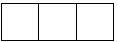
\includegraphics{figures/straight_trominoe.pdf}%
\end{picture}%
\setlength{\unitlength}{3947sp}%
%
\begingroup\makeatletter\ifx\SetFigFont\undefined%
\gdef\SetFigFont#1#2#3#4#5{%
  \reset@font\fontsize{#1}{#2pt}%
  \fontfamily{#3}\fontseries{#4}\fontshape{#5}%
  \selectfont}%
\fi\endgroup%
\begin{picture}(924,324)(1189,-673)
\end{picture}%
 and L-shaped 
\begin{picture}(0,0)%
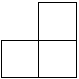
\includegraphics{figures/L-shaped_trominoe.pdf}%
\end{picture}%
\setlength{\unitlength}{3947sp}%
%
\begingroup\makeatletter\ifx\SetFigFont\undefined%
\gdef\SetFigFont#1#2#3#4#5{%
  \reset@font\fontsize{#1}{#2pt}%
  \fontfamily{#3}\fontseries{#4}\fontshape{#5}%
  \selectfont}%
\fi\endgroup%
\begin{picture}(624,624)(1189,-673)
\end{picture}%
. This problem is only concerned with
the L-shaped trominoes.)
\end{enumerate}

\hint{If $n=1$ we have: ``Every $2 \times 2$ chessboard -- with one square removed
can be tiled perfectly by L-shaped trominoes.  This version is trivial to prove.  Try formulating
the $n=0$ case.}

\wbvfill
  
\hintspagebreak
\workbookpagebreak

\item Suppose that the rules of the game for PMI were changed so that one
did the following:
\begin{itemize}
\item Basis.  Prove that $P(0)$ is true.
\item Inductive step.  Prove that for all $k$, $P_k$ implies $P_{k+2}$
\end{itemize}


\noindent Explain why this would not constitute a valid proof that $P_n$ holds 
for all natural numbers $n$. 
\noindent How could we change the basis in this outline to obtain a valid proof?

\hint{In this modified version, $P(0)$ is not going to imply $P(1)$. and in fact, none of the odd numbered
statements will be proven.  If we change the 
basis so that we prove both $P(0$ and $P(1)$, all the even statements will be implied by
$P(0$ being true and all the odd statements get forced because $P(1)$ is true.}

\wbvfill

\item If we wanted to prove statements that were indexed by the integers,

\[ \forall z \in \Integers, \; P_z, \]

\noindent what changes should be made to PMI?

\hint{A quick change would be to replace $\forall k, \; P_k \implies P_{k+1}$ in the inductive
step with $\forall k, \; P_k \iff P_{k+1}$.  While this would do the trick, a slight improvement 
is possible, if we treat the positive and negative cases for $k$ separately.}

 \wbvfill
 
 \workbookpagebreak
 
\end{enumerate}


%% Emacs customization
%% 
%% Local Variables: ***
%% TeX-master: "GIAM-hw.tex" ***
%% comment-column:0 ***
%% comment-start: "%% "  ***
%% comment-end:"***" ***
%% End: ***

